
% =================================================================================
% Informationen (Meta-Daten) f�r pdf
% =================================================================================
\hypersetup{
	pdftitle = {},
	pdfsubject = {},
	pdfkeywords = {},
	pdfcreator = {},
	pdfproducer = {LaTeX with hyperref},
	pdfstartview = {Fit},
	pdfpagelayout = {SinglePage}
}
% =================================================================================


% =================================================================================
% Theorem-Definitionen
% =================================================================================
\ifReport
	\newtheorem{theorem}{Satz}
	\newtheorem{lemma}[theorem]{Lemma}
	\newtheorem{definition}{Definition}
	
	\newtheorem{example}{Beispiel}
\fi
% =================================================================================


%% =================================================================================
%% Umgebungen f�r Aufgabe
%% =================================================================================
%\newcounter{problemnb}[part]      % Neuer Counter bspnummer nummeriert nach Kapitel
%\def\theproblemnb{\thepart.\arabic{problemnb}}
%
%\makeatletter	% Definiert "`@"'-Zeichen um (n�tig f�r \@beginparpenalty)
%\newenvironment{problemexp}%
%	{\refstepcounter{problemnb}%	% Aufgabennummer inkrementieren
%		\vspace{2ex}				% Etwas Platz vor Aufgabe
%		\@beginparpenalty=10000%	% Vor Liste auf keinen Fall umbrechen
%%									% (verhindert, dass "`Aufgabe ..."' alleine
%%									% am Fu� einer Seite steht, und alles andere
%%									% dann auf der n�chsten
%		\par%						% Zeilenumbruch erzwingen
%		\noindent%					% Keinen Einzug
%		\textbf{Aufgabe \theproblemnb\ (Durchf�hrung/Nachbearbeitung):}%
%		\begin{itemize}}%
%	{\end{itemize}%
%		\vspace{3ex}}
%\makeatother	% "`@"'-Zeichen wieder normal
%
%\makeatletter 
%\newenvironment{problemprep}%
%{\refstepcounter{problemnb} \vspace{2ex} \@beginparpenalty=10000 \par \noindent \textbf{Aufgabe \theproblemnb\ (Vorbereitung):}\begin{itemize}}%
%{\end{itemize}\vspace{3ex}}
%\makeatother
%% =================================================================================
%
%
%% =================================================================================
%% Umgebungen f�r L�sung
%% =================================================================================
%\newcommand{\solutionframed}[1]{%
%	\ifSolution %
%		\begin{framed}%
%			\noindent \textbf{L�sung:}\\%
%			#1 %
%		\end{framed}%
%	\fi }
%
%\newcommand{\solutioncomment}[1]{%
%	\ifSolution %
%		\begin{framed}%
%			#1 %
%		\end{framed}%
%	\fi }
%
%
%\makeatletter 
%\newenvironment{solution}[1]%
%{\vspace{2ex} \@beginparpenalty=10000 \par \noindent \textbf{L�sung zu Aufgabe~\ref{#1}:}\begin{itemize}}%
%{\end{itemize}\vspace{3ex}}
%\makeatother
%% =================================================================================


% =================================================================================
% Definitionen f�r pgfplot
% =================================================================================

%\pgfplotsset{compat=1.3}

\pgfplotsset{x tick label style={/pgf/number format/use comma, /pgf/number format/1000 sep=\,},
				y tick label style={/pgf/number format/use comma, /pgf/number format/1000 sep=\,},
				z tick label style={/pgf/number format/use comma, /pgf/number format/1000 sep=\,},
				every axis legend/.append style={nodes={right}},
				every axis/.append style={line width=0ex,solid}}

\pgfplotsset{
	/pgfplots/xlabel near ticks/.style={
		/pgfplots/every axis x label/.style={
			at={(ticklabel cs:0.5)},anchor=near ticklabel
		}
	},
	/pgfplots/ylabel near ticks/.style={
		/pgfplots/every axis y label/.style={
			at={(ticklabel cs:0.5)},rotate=90,anchor=near ticklabel
		}
	}
}

\pgfplotsset{every axis/.append style={line width=.5pt},
				every tick/.append style={line width=0.5pt, black}}
				
%\pgfplotsset{every legend/.append style={/tikz/every row/.append style={row sep=0cm}}}


\pgfplotsset{
		cycle list = {{blue,style=solid}, {red, style=dashed}, {olive,style=solid}, %
						{black,style=dashed}, {purple,style=solid}, {orange,style=dashed}}
}


%\pgfplotsset{
%   mein overlay style/.style={
%    ylabel style={overlay},
%    yticklabel style={overlay}
%  }
%}

% =================================================================================


\tikzstyle{block} = [draw,rectangle,thick,minimum height=2em,minimum width=2em]
\tikzstyle{hblock} = [draw,rectangle,thick,minimum height=3em,minimum width=2em]
\tikzstyle{Hblock} = [draw,rectangle,thick,minimum height=4em,minimum width=2em]
\tikzstyle{sum} = [draw,circle,inner sep=0mm,minimum size=2mm]
\tikzstyle{line} = [semithick]
\tikzstyle{branch} = [circle,inner sep=0pt,minimum size=1mm,fill=black,draw=black]
\tikzstyle{guide} = []
\tikzstyle{connector} = [->,semithick]

\tikzstyle{flowenterexit} = [draw, rounded rectangle, thick, text badly centered, text width=4.5cm]
\tikzstyle{flowsub} = [draw, double, thick, text width = 4cm, minimum height=1.5cm, text centered]
\tikzstyle{flowcond} = [draw, diamond, shape aspect = 2, thick, text badly centered, inner sep=0pt, minimum width=4.5cm, minimum height=1.5cm]
\tikzstyle{flowaction} = [draw, thick, text width = 4cm, minimum height=1.5cm, text centered]
 

\newcommand{\TikZsaturation}{
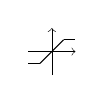
\begin{tikzpicture}
	% Koordinatensystem
	\draw[->, very thin] (-3mm,0) -- (3mm,0);
	\draw[->, very thin] (0,-3mm) -- (0,3mm);

	% Saturation
	\draw[thin] (-3mm,-1.5mm) -- (-1.5mm,-1.5mm);
	\draw[thin] (-1.5mm,-1.5mm) -- ( 1.5mm, 1.5mm);
	\draw[thin] ( 1.5mm, 1.5mm) -- ( 3mm, 1.5mm);
\end{tikzpicture}
}
%\begin{tikzpicture}
	%% Koordinatensystem
	%\draw[->, very thin] (-3mm,0) -- (3mm,0);
	%\draw[->, very thin] (0,-3mm) -- (0,3mm);
%
	%% Saturation
	%\draw[thin] (-3mm,-1.875mm) -- (-0.75mm,-1.875mm);
	%\draw[thin] (-0.75mm,-1.875mm) -- ( 0.75mm, 1.875mm);
	%\draw[thin] ( 0.75mm, 1.875mm) -- ( 3mm, 1.875mm);
%\end{tikzpicture}
% =================================================================================
% Definitionen f�r Listingsumgebung
% =================================================================================

\lstloadlanguages{Matlab}

\lstdefinestyle{Matlab_colored_smallfont}
{
	language = Matlab,
	tabsize = 4,
	framesep = 3mm,
	frame=tb,
	classoffset = 0,	
	basicstyle = \footnotesize\ttfamily,
	keywordstyle = \bfseries\color[rgb]{0,0,1},
	commentstyle = \itshape\color[rgb]{0.133,0.545,0.133},
	stringstyle = \color[rgb]{0.627,0.126,0.941},
	extendedchars = true,
	breaklines = true,
	prebreak = \textrightarrow,
	postbreak = \textleftarrow,
	%escapeinside = {(*@}{@*)},
	%moredelim = [s][\itshape\color[rgb]{0.5,0.5,0.5}]{[.}{.]},
	numbers = left,
	numberstyle = \tiny,
	stepnumber = 5
}
 
\lstdefinestyle{Matlab_colored}
{
	language = Matlab,
	tabsize = 4,
	framesep = 3mm,
	frame=tb,
	classoffset = 0,	
	basicstyle = \ttfamily,
	keywordstyle = \bfseries\color[rgb]{0,0,1},
	commentstyle = \itshape\color[rgb]{0.133,0.545,0.133},
	stringstyle = \color[rgb]{0.627,0.126,0.941},
	extendedchars = true,
	breaklines = true,
	prebreak = \textrightarrow,
	postbreak = \textleftarrow,
	%escapeinside = {(*@}{@*)},
	%moredelim = [s][\itshape\color[rgb]{0.5,0.5,0.5}]{[.}{.]},
	numbers = left,
	numberstyle = \tiny,
	stepnumber = 5
}                


\lstdefinestyle{C_colored_smallfont}
{
	language=C,
	tabsize = 4,
	framesep = 3mm,
	frame=tb,	
	classoffset = 0,	
	basicstyle = \footnotesize\ttfamily,
	keywordstyle = \bfseries\color[rgb]{0,0,1},
	commentstyle = \itshape\color[rgb]{0.133,0.545,0.133},
	stringstyle = \color[rgb]{0.627,0.126,0.941},
	extendedchars = true,
	breaklines = true,
	prebreak = \textrightarrow,
	postbreak = \textleftarrow,
	%escapeinside = {(*@}{@*)},
	%moredelim = [s][\itshape\color[rgb]{0.5,0.5,0.5}]{[.}{.]},
	numbers = left,
	numberstyle = \tiny,
	stepnumber = 5
}

\lstdefinestyle{C_colored}
{
	language=C,
	tabsize = 4,
	framesep = 3mm,
	frame=tb,
	classoffset = 0,	
	basicstyle = \ttfamily,
	keywordstyle = \bfseries\color[rgb]{0,0,1},
	commentstyle = \itshape\color[rgb]{0.133,0.545,0.133},
	stringstyle = \color[rgb]{0.627,0.126,0.941},
	extendedchars = true,
	breaklines = true,
	prebreak = \textrightarrow,
	postbreak = \textleftarrow,
	%escapeinside = {(*@}{@*)},
	%moredelim = [s][\itshape\color[rgb]{0.5,0.5,0.5}]{[.}{.]},
	numbers = left,
	numberstyle = \tiny,
	stepnumber = 5
}
